\begin{frame}
    \frametitle{Testy}

    Rodzaje modeli
    \begin{enumerate}
        \item Model podstawowy
        \begin{enumerate}
            \item uczony na grafach czterowierzchołkowych
            \item uczony na grafach pięciowierzchołkowych
            \item uczony na grafach sześciowierzchołkowych
            \item uczony na grafach siedmiowierzchołkowych
        \end{enumerate}
        \item Model z walidacją krzyżową
        \begin{enumerate}
            \item wersja podstawowa
            \item wersje z pojedynczymi modyfikacjami
            \item wersja zmodyfikowana
        \end{enumerate}
        \item Model ze zmienną liczbą wierzchołków
        \begin{enumerate}
            \item wersja podstawowa
            \item wersje z pojedynczymi modyfikacjami
            \item wersja zmodyfikowana
        \end{enumerate}
        \item Model ze zmienną liczbą wierzchołków i walidacją krzyżową
        \begin{enumerate}
            \item wersja podstawowa
            \item wersje z pojedynczymi modyfikacjami
            \item wersja zmodyfikowana
        \end{enumerate}
    \end{enumerate}
    
\end{frame}

\begin{frame}
    \frametitle{Testy}

    Rodzaje modyfikacji
    \begin{enumerate}
        \item Liczba filtrów w~warstwach Conv2D oraz parametr Dropout.
        \item Normalizacja wsadowa pomiędzy warstwami modelu.
        \item Augmentacja danych przed budową modelu.
        \item Zmniejszenie szybkości uczenia.
    \end{enumerate}
    
\end{frame}


\begin{frame}
    \frametitle{Testy}

    \begin{figure}[ht]
        \centering
        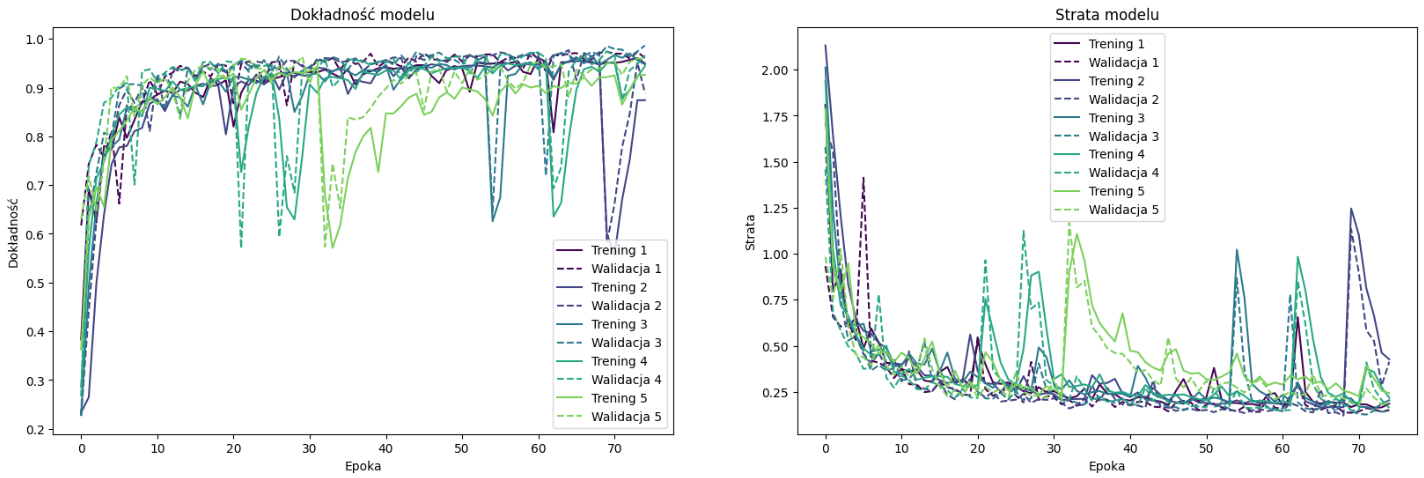
\includegraphics[width=10cm]{../thesis/resources/tests/images/v3/crossvalid_img.png}
        \caption{Wyniki testów dla modelu z~walidacją krzyżową}
    \end{figure}
    
\end{frame}

\begin{frame}
    \frametitle{Testy}

    \begin{figure}[ht]
        \centering
        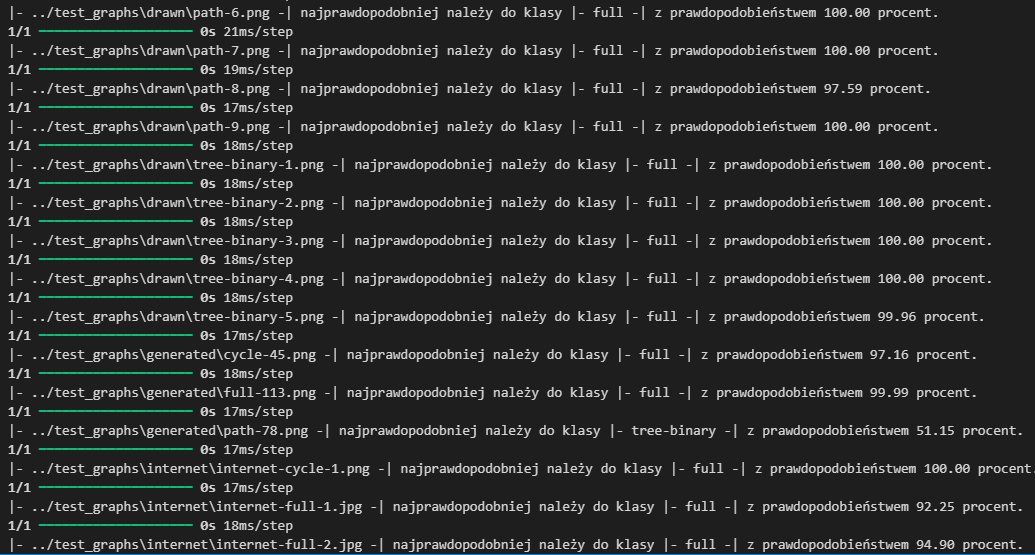
\includegraphics[width=10cm]{../thesis/resources/tests/images/v3/crossvalid_txt.png}
        \caption{Klasyfikacja obrazów zewnętrznych dla modelu z~walidacją krzyżową}
    \end{figure}

\end{frame}

\begin{frame}
    \frametitle{Testy}

    \begin{figure}[ht]
        \centering
        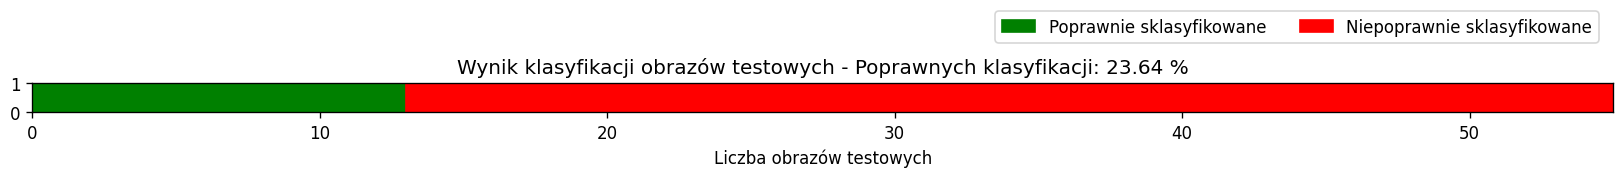
\includegraphics[width=11cm]{../thesis/resources/tests/images/v3/crossvalid_bar.png}
        \caption{Wizualizacja klasyfikacji obrazów zewnętrznych dla modelu z~walidacją krzyżową}
    \end{figure}
    
    \begin{figure}[ht]
        \centering
        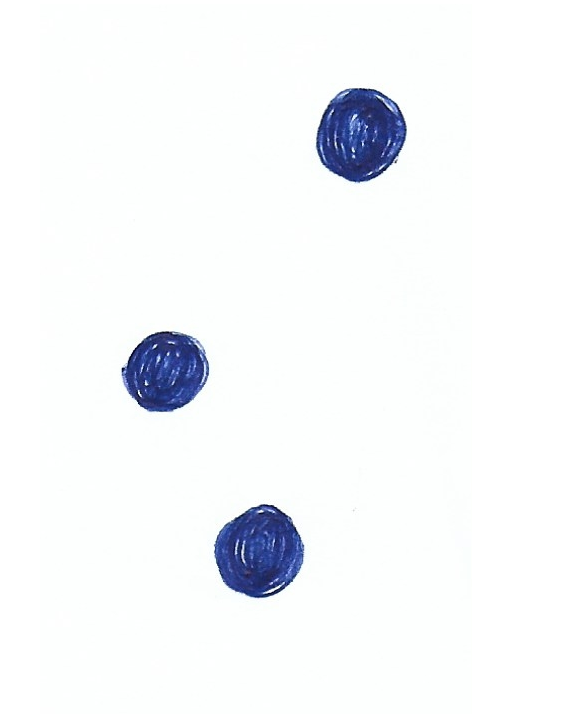
\includegraphics[height=2cm]{../graph_classification/test_graphs/drawn/empty-1.png}
        \caption{Klasyfikacja przykładowego grafu zewnętrznego przez model z~walidacją krzyżową.
            Przypisana klasa to~graf pełny z~99,62\% pewnością.
            Biorąc pod uwagę wysoką pewność przy klasyfikacji,
            można by spodziewać się lepszego wyniku niż otrzymany nieprawidłowy.}
    \end{figure}

\end{frame}

